%%%%%%%%%%%%%%%%%%%%%%%% EXPERIMENTS %%%%%%%%%%%%%%%%%%%%%%%%%%%%%%%%%%%%%%%%
% All experiment-related floats (Tables 1-6 and figure) live inside \section{Experiments} below.
%===============================================================================

\section{Experiments}
\label{sec:result}

We evaluate whether CRAPE can turn code-generated trajectories into effective real-world supervision for VLA fine-tuning. 
The experiments are designed to test three central claims: 
CRAPE can approach human teleoperation performance, outperform vanilla code-based data collection, and transfer across VLA backbones and robot embodiments. 
We further ablate its main components to isolate the roles of state-coverage seeding and pre-selective acquisition.

% \section{Experiments}
% \label{sec:result}
% We evaluate whether CRAPE can turn code-generated trajectories into effective real-world VLA supervision. 
% Our experiments ask four questions: 
% \textbf{(RQ1)} Can CRAPE-collected data train policies that match human teleoperation? 
% \textbf{(RQ2)} Does pre-selective acquisition produce more learnable data than vanilla code-based collection? 
% \textbf{(RQ3)} Which components of CRAPE are necessary? 
% \textbf{(RQ4)} Does the benefit transfer across VLA backbones and robot embodiments?
% RQ3의 OOD/robustness 측면은 Main Results의 jitter 환경 SR과 Ablation의 perturbation 제거 조건에 흡수됨.

%---------------------------------------------------------------
\subsection{Experimental Setup}
\label{sec:setup}

\textbf{Benchmark.}
We construct a real-world benchmark of 10 manipulation tasks covering pick-and-place, distribution, sorting, stacking, articulated lid/drawer manipulation, multi-step arrangement, and deformable bimanual manipulation: 
\textit{pick\_place}~(T1), \textit{distribute\_bread}~(T2), \textit{sort3}~(T3), \textit{stack3}~(T4), \textit{close\_pot}~(T5), \textit{open\_drawer}~(T6), \textit{prepare\_meal}~(T7), \textit{fold\_towel}~(T8), \textit{open\_lid}~(T9), and \textit{close\_drawer}~(T10). 
The main benchmark uses the SO-101 platform, with a dual-SO-101 setup; cross-embodiment results on UR7e are reported in Table~\ref{tab:crossembod}.

\textbf{Baselines.}
We compare CRAPE against three data-collection baselines: human teleoperation; RoboTwin~\citep{chen2025robotwin}, a code-based simulation pipeline whose code-generation scheme we port to real-world collection; and Manipulate-Anything (MA)~\citep{duan2024manipulate}, a VLM-driven open-loop real-world baseline.

\textbf{Training and evaluation.}
All methods use the same LLM-generated primitive skill library and the same Isaac~Lab sim-pretraining stage before real-world fine-tuning. 
We evaluate two VLA backbones, smolVLA and GR00T~N1.5~\citep{bjorck2025gr00t,nvidiagear2025gr00tn15}, each fine-tuned per task under the same protocol. 
Each trained policy is evaluated over 30 rollouts under matched initial conditions using task-specific success criteria. 
Fine-tuning consumed approximately \textit{250} GPU-hours on H100 GPUs.

% =================================================================
% [Table 1] Main Results: 4 collection methods x 2 VLAs x 10 tasks
% =================================================================
\begin{table*}[t]
\label{tab:main}
\centering

\caption{Main results on the real-world benchmark. We measure success rate (\%) over 10 manipulation tasks for two VLA backbones trained under an same fine-tune procedure.}

\small
\setlength{\tabcolsep}{3pt}
\begin{tabular}{ll cccccccccc c}
\toprule
\textbf{Method} & \textbf{VLA}
& \textbf{T1} & \textbf{T2} & \textbf{T3} & \textbf{T4} & \textbf{T5}
& \textbf{T6} & \textbf{T7} & \textbf{T8} & \textbf{T9} & \textbf{T10}
& \textbf{Overall} \\
\midrule
\multirow{2}{*}{Teleoperation}
  & smolVLA     & 83.33 & 66.67 & 0 & 0 & 6.67 & 96.67 & 50.00 & -- & 93.33 & 93.33 & -- \\
  & GR00T N1.5  & 40.00 & 26.67 & 0 & 0 & 0 & 76.67 & 36.67 & -- & 0 & 100 & -- \\
\midrule
\multirow{2}{*}{RoboTwin}
  & smolVLA     & 0 & 0 & 0 & 0 & 56.67 & 100 & 3.33 & -- & 6.67 & 0 & -- \\
  & GR00T N1.5  & 13.33 & 0 & 0 & 0 & 0 & 96.67 & 23.33 & -- & 0 & 13.33 & -- \\
\midrule
\multirow{2}{*}{MA}
  & smolVLA     & 0 & 0 & 13.33 & 0 & 63.33 & 100 & 0 & -- & 0 & 0 & -- \\
  & GR00T N1.5  & 6.67 & 0 & 0 & 0 & 0 & 93.33 & 30.00 & -- & 0 & 26.67 & -- \\
\midrule
\multirow{2}{*}{\textbf{CRAPE (Ours)}}
  & smolVLA     & 100 & 0 & 33.33 & 6.67 & 33.33 & 100 & 96.67 & -- & 100 & 86.67 & -- \\
  & GR00T N1.5  & 23.33 & 0 & 0 & 0 & 53.33 & 100 & 100 & -- & 0 & 93.33 & -- \\
\bottomrule
\end{tabular}
\end{table*}

%---------------------------------------------------------------
% \subsection{Main Results}
% \label{sec:exp_main}

% The main results shows whether CRAPE-collected data can serve as effective real-world supervision for VLA fine-tuning, matching human teleoperation while outperforming vanilla code-based collection. 
% Table~\ref{tab:main} reports success rates across 10 tasks, four collection methods, and two VLA backbones under the same sim-pretrain and real-world fine-tune protocol. 
% All methods use an identical Isaac~Lab sim-pretraining stage before real-world fine-tuning, which equalizes the starting point across methods and isolates the effect of real-world data acquisition.

% \textbf{Teleoperation-level performance.}
% CRAPE achieves success rates comparable to policies trained on human teleoperation across the benchmark. 
% This indicates that code-generated trajectories can replace much of the manual demonstration burden when they are selectively acquired as clean and informative VLA supervision.

% \textbf{Comparison to vanilla code-based collection.}
% RoboTwin~2.0 and Manipulate-Anything often generate feasible real-world rollouts, but their unfiltered trajectories are less effective for closed-loop VLA training. 
% Policies trained on these data are more brittle under actuation jitter and small state deviations, suggesting that executable demonstrations are not necessarily learnable demonstrations. 
% CRAPE improves over these baselines by selecting trajectories that expand coverage while remaining locally consistent with the existing buffer.

% \textbf{Consistency across VLA backbones.}
% The same trend holds for both smolVLA and GR00T~N1.5, showing that CRAPE's gains are not tied to a specific policy architecture. 
% Rather, the improvement comes from the quality of the acquired data: state-coverage seeding provides clean support, and pre-selective acquisition admits candidates that are diverse, consistent, and informative.
% % \subsection{Main Results}
% % \label{sec:exp_main}

% % Table~\ref{tab:main} reports per-task and overall SR for all four collection
% % methods across the two VLA backbones, targeting three aims:
% % (i)~SR competitiveness against human teleoperation,
% % (ii)~superiority over vanilla code-based collection (RoboTwin, MA), and
% % (iii)~generality across off-the-shelf VLA backbones.

% % \textbf{Protocol specific to this experiment.}
% % All methods share an identical sim-pretraining stage on Isaac~Lab
% % demonstrations before real-world fine-tuning; without it, RoboTwin- and
% % MA-collected data alone drive the policy into states from which it cannot
% % recover, so sim-pretraining equalizes the floor across methods.

% % \textbf{(RQ1) CRAPE matches human teleoperation.}
% % Across the 10 tasks, policies trained on CRAPE-collected data reach overall
% % SR comparable to human teleoperation.

% % \textbf{(RQ2) Vanilla code-based collection fails to transfer to the real world.}
% % Despite the shared sim-pretraining stage, RoboTwin- and MA-trained policies yield
% % low SR (overall \textit{XX\%}); SO-101's actuation jitter repeatedly drives
% % the policy out-of-distribution. Vanilla code-based collection is therefore
% % unfit for real-world VLA training.

% % \textbf{(RQ3) The CRAPE recipe generalizes across VLAs.}
% % Phase~1 canonical subgoal seeding broadens state coverage, and Phase~2
% % pre-selective acquisition admits only useful trajectories, producing a VLA
% % that is robust to jitter-induced OOD while remaining consistent in its
% % predictions. The pattern is preserved across both smolVLA and GR00T~N1.5,
% % confirming that the advantage is a property of the collected data.

% % =================================================================
% %========================== CHANGED ↓ : Data Quality (scatter + trend figures + narrative; replaces former Table 2) ==========================
% % Data Quality & Sample Efficiency — visualized as two figures:
% %   fig:quality_scatter (100ep snapshot, diversity vs NCD)
% %   fig:quality_trend   (scaling over 20-100 episodes, mean +/- std over tasks)
% % =================================================================

% \begin{figure}[t]
%   \centering
%   \includegraphics[width=\linewidth]{figure/traj_visualization.png}
%   \caption{Per-task diversity (Signature) vs.\ diversity-invariant consistency (NCD) at $100$ episodes. Each marker is a task; shading is per-method hdensity. Higher on the plot is more consistent.}
%   \label{fig:traj_visualization}
%   \vspace{-0.1in}
% \end{figure}



% \begin{figure}[t]
%   \centering
%   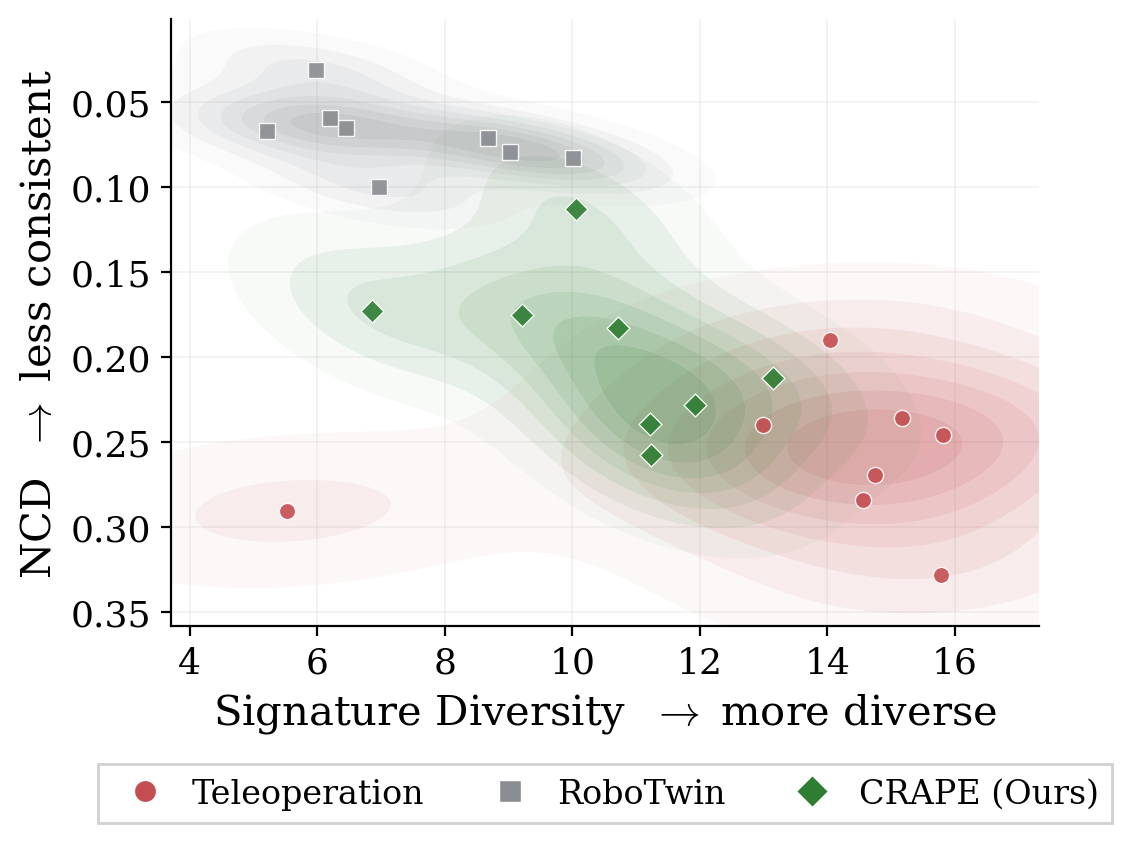
\includegraphics[width=0.66\linewidth]{figure/fig_quality_scatter.png}
%   \caption{Per-task diversity (Signature) vs.\ diversity-invariant consistency (NCD) at $100$ episodes. Each marker is a task; shading is per-method hdensity. Higher on the plot is more consistent.}
%   \label{fig:quality_scatter}
%   \vspace{-0.1in}
% \end{figure}

% \begin{figure*}[t]
%   \centering
%   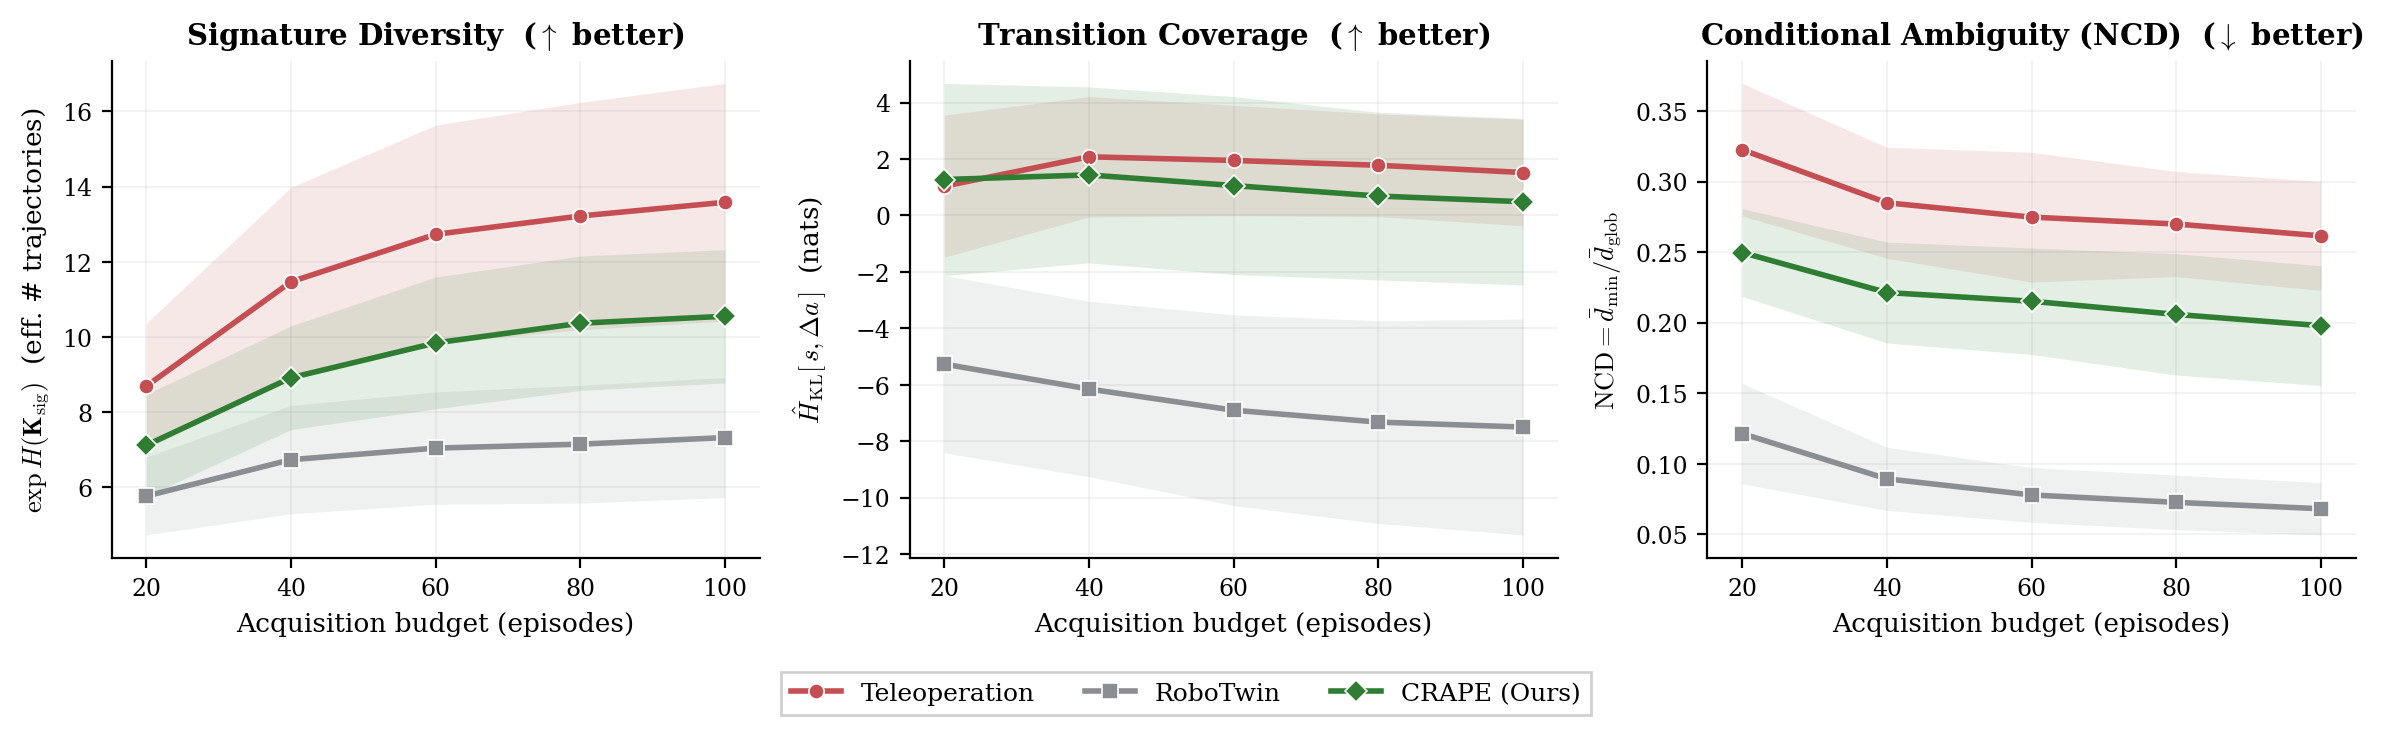
\includegraphics[width=\textwidth]{figure/fig_quality_trend.png}
%   \caption{Dataset quality vs.\ acquisition budget. Lines: mean over the $8$ single-arm tasks; bands: $\pm 1$ std across tasks.}
%   \label{fig:quality_trend}
%   \vspace{-0.15in}
% \end{figure*}

% %---------------------------------------------------------------
% \subsection{Data Quality and Sample Efficiency}
% \label{sec:exp_quality}

% Figures~\ref{fig:quality_scatter} and~\ref{fig:quality_trend} ask whether CRAPE's gains come from collecting \emph{more} episodes or \emph{more learnable} ones, tracking diversity, coverage, and NCD as the acquisition budget grows ($20\!\to\!100$ episodes).

% CRAPE is the only method whose dataset quality and SR improve together with scale. It raises Signature Diversity and Transition Coverage toward teleoperation level (Ours $10.6$/$0.5$ vs.\ RoboTwin $7.3$/$\!-\!7.5$ at $100$ episodes) while keeping conditional ambiguity low \emph{relative to its diversity}. RoboTwin saturates under the same budget: its deterministic primitives make extra rollouts redundant, so executable rollouts are not learnable supervision.

% Because diversity and raw consistency trade off, we measure consistency with NCD (local ambiguity normalized by global diversity). Teleoperation is diverse but comparatively inconsistent---heterogeneous human action modes give it high conditional ambiguity---whereas CRAPE attains \emph{lower} ambiguity on all $8$ single-arm tasks (NCD; Wilcoxon $p=0.004$, mean gap $0.063$, $95\%$ CI $[0.034,0.091]$). Figure~\ref{fig:quality_scatter} summarizes the trade-off at $100$ episodes: RoboTwin occupies the low-diversity region, teleoperation the high-diversity/high-ambiguity region, and CRAPE the desired high-diversity/low-ambiguity ``useful-diversity'' regime. These advantages strengthen with the acquisition budget (Figure~\ref{fig:quality_trend}): CRAPE's diversity keeps growing while RoboTwin saturates, and NCD improves at every budget with CRAPE more consistent than teleoperation throughout---CRAPE collects \emph{more learnable}, not merely more, data.

\subsection{Main Results}
\label{sec:exp_main}

The main results shows whether CRAPE-collected data can serve as effective real-world supervision for VLA fine-tuning, matching human teleoperation while outperforming vanilla code-based collection.
Table~\ref{tab:main} reports success rates across 10 tasks, four collection methods, and two VLA backbones under the same sim-pretrain and real-world fine-tune protocol.
All methods use an identical Isaac~Lab sim-pretraining stage before real-world fine-tuning, which equalizes the starting point across methods and isolates the effect of real-world data acquisition.

\textbf{Teleoperation-level performance.}
CRAPE achieves success rates comparable to policies trained on human teleoperation across the benchmark.
This indicates that code-generated trajectories can replace much of the manual demonstration burden when they are selectively acquired as clean and informative VLA supervision.

\textbf{Comparison to vanilla code-based collection.}
RoboTwin~2.0 and Manipulate-Anything often generate feasible real-world rollouts, but their unfiltered trajectories are less effective for closed-loop VLA training.
Policies trained on these data are more brittle under actuation jitter and small state deviations, suggesting that executable demonstrations are not necessarily learnable demonstrations.
CRAPE improves over these baselines by selecting trajectories that expand coverage while remaining locally consistent with the existing buffer.

\textbf{Consistency across VLA backbones.}
The same trend holds for both smolVLA and GR00T~N1.5, showing that CRAPE's gains are not tied to a specific policy architecture.
Rather, the improvement comes from the quality of the acquired data: state-coverage seeding provides clean support, and pre-selective acquisition admits candidates that are diverse, consistent, and informative.
% \subsection{Main Results}
% \label{sec:exp_main}

% Table~\ref{tab:main} reports per-task and overall SR for all four collection
% methods across the two VLA backbones, targeting three aims:
% (i)~SR competitiveness against human teleoperation,
% (ii)~superiority over vanilla code-based collection (RoboTwin, MA), and
% (iii)~generality across off-the-shelf VLA backbones.

% \textbf{Protocol specific to this experiment.}
% All methods share an identical sim-pretraining stage on Isaac~Lab
% demonstrations before real-world fine-tuning; without it, RoboTwin- and
% MA-collected data alone drive the policy into states from which it cannot
% recover, so sim-pretraining equalizes the floor across methods.

% \textbf{(RQ1) CRAPE matches human teleoperation.}
% Across the 10 tasks, policies trained on CRAPE-collected data reach overall
% SR comparable to human teleoperation.

% \textbf{(RQ2) Vanilla code-based collection fails to transfer to the real world.}
% Despite the shared sim-pretraining stage, RoboTwin- and MA-trained policies yield
% low SR (overall \textit{XX%}); SO-101's actuation jitter repeatedly drives
% the policy out-of-distribution. Vanilla code-based collection is therefore
% unfit for real-world VLA training.

% \textbf{(RQ3) The CRAPE recipe generalizes across VLAs.}
% Phase~1 canonical subgoal seeding broadens state coverage, and Phase~2
% pre-selective acquisition admits only useful trajectories, producing a VLA
% that is robust to jitter-induced OOD while remaining consistent in its
% predictions. The pattern is preserved across both smolVLA and GR00T~N1.5,
% confirming that the advantage is a property of the collected data.

% =================================================================
%========================== CHANGED ↓ : Data Quality (scatter + trend figures + narrative; replaces former Table 2) ==========================
% Data Quality & Sample Efficiency — visualized as two figures:
%   fig:quality_scatter (100ep snapshot, diversity vs NCD)
%   fig:quality_trend   (scaling over 20-100 episodes, mean +/- std over tasks)
% =================================================================

\begin{figure}[t]
\centering
\includegraphics[width=\linewidth]{figure/traj_visualization.png}
\caption{Per-task diversity (Signature) vs.\ diversity-invariant consistency (NCD) at $100$ episodes. Each marker is a task; shading is per-method hdensity. Higher on the plot is more consistent.}
\label{fig:traj_visualization}
\vspace{-0.1in}
\end{figure}

\begin{figure*}[t]
\centering
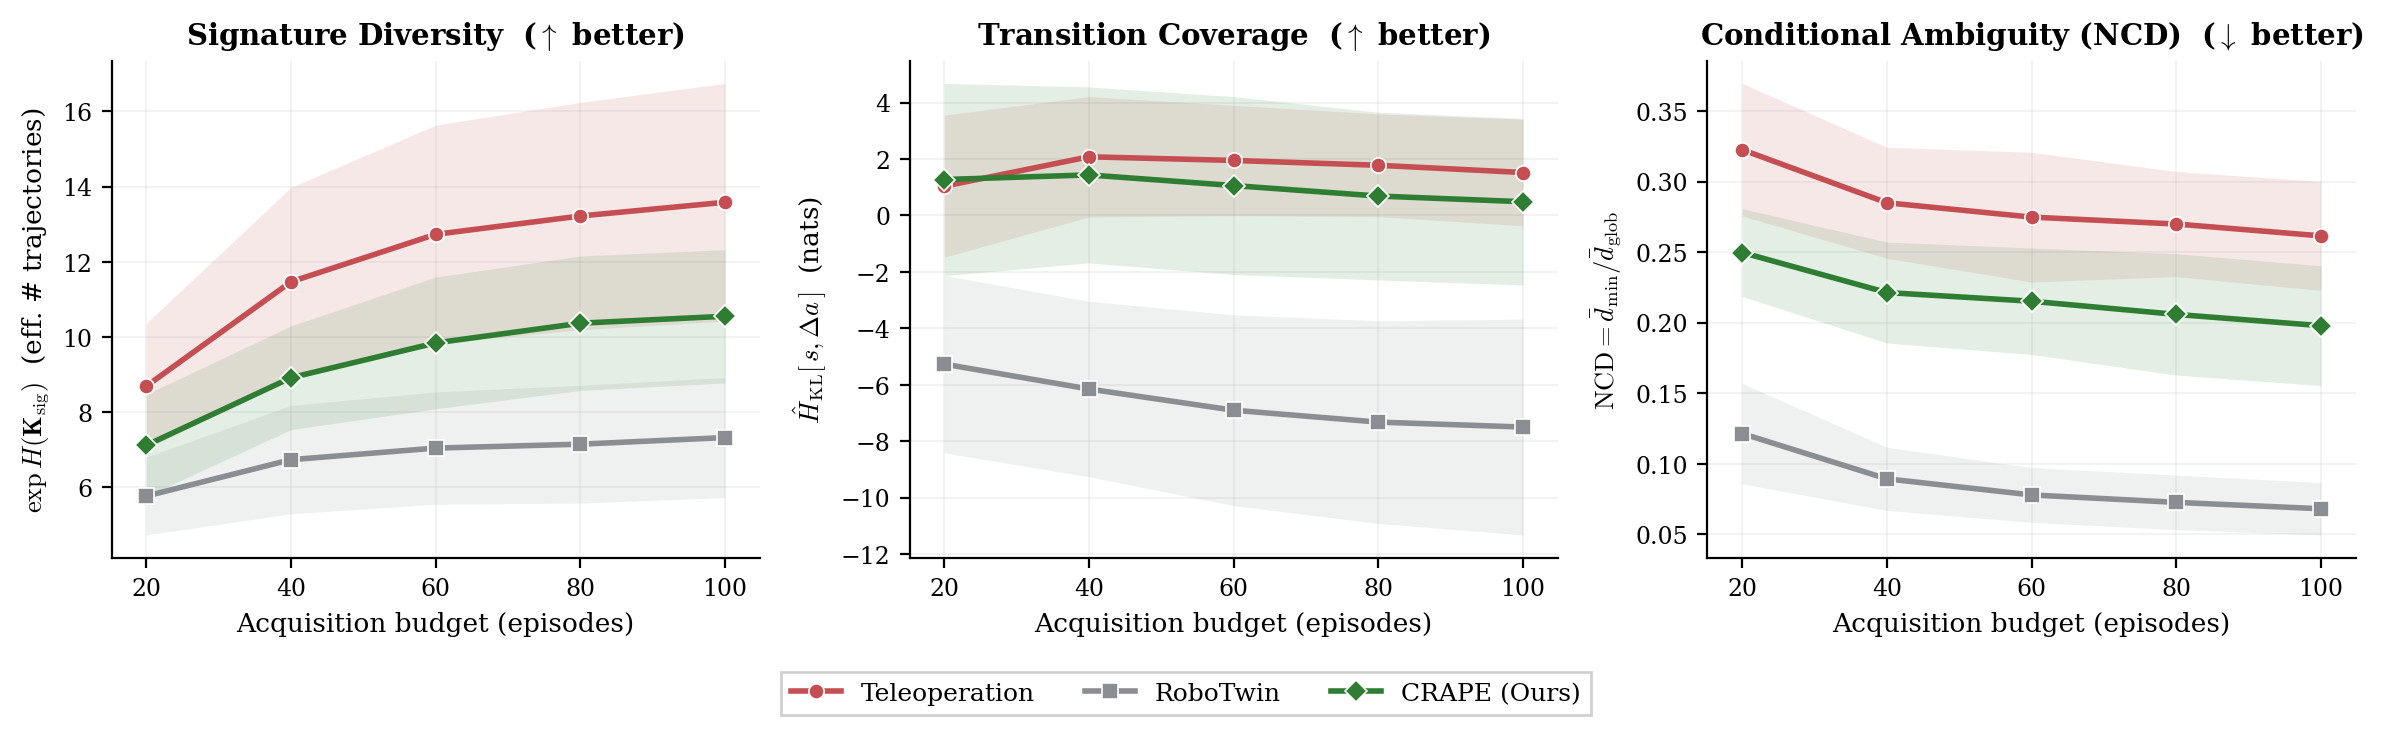
\includegraphics[width=\textwidth]{figure/fig_quality_trend.png}
\caption{Dataset quality vs.\ acquisition budget. Lines: mean over the $8$ single-arm tasks; bands: $\pm 1$ std across tasks.}
\label{fig:quality_trend}
\vspace{-0.15in}
\end{figure*}

%---------------------------------------------------------------
\subsection{Data Quality and Sample Efficiency}
\label{sec:exp_quality}

Figures~\ref{fig:quality_scatter} and~\ref{fig:quality_trend} ask whether CRAPE's gains come from collecting \emph{more} episodes or \emph{more learnable} ones, tracking diversity, coverage, and NCD as the acquisition budget grows ($20!\to!100$ episodes).

CRAPE is the only method whose dataset quality and SR improve together with scale. It raises Signature Diversity and Transition Coverage toward teleoperation level (Ours $10.6$/$0.5$ vs.\ RoboTwin $7.3$/$!-!7.5$ at $100$ episodes) while keeping conditional ambiguity low \emph{relative to its diversity}. RoboTwin saturates under the same budget: its deterministic primitives make extra rollouts redundant, so executable rollouts are not learnable supervision.

Because diversity and raw consistency trade off, we measure consistency with NCD (local ambiguity normalized by global diversity). Teleoperation is diverse but comparatively inconsistent---heterogeneous human action modes give it high conditional ambiguity---whereas CRAPE attains \emph{lower} ambiguity on all $8$ single-arm tasks (NCD; Wilcoxon $p=0.004$, mean gap $0.063$, $95\%$ CI $[0.034,0.091]$). Figure~\ref{fig} summarizes the trade-off at $100$ episodes: RoboTwin occupies the low-diversity region, teleoperation the high-diversity/high-ambiguity region, and CRAPE the desired high-diversity/low-ambiguity ``useful-diversity'' regime. These advantages strengthen with the acquisition budget (Figure~\ref{fig}): CRAPE's diversity keeps growing while RoboTwin saturates, and NCD improves at every budget with CRAPE more consistent than teleoperation throughout---CRAPE collects \emph{more learnable}, not merely more, data.



% \subsection{Data Quality and Sample Efficiency}
% \label{sec:exp_quality}

% Table~\ref{tab:quality} tracks four dataset-level quality metrics and downstream SR as episodes grow ($30/50/100$) over a common pool of 10 fixed layouts. The central claim is \emph{joint}: useful diversity means expanding action coverage while keeping local actions consistent, which only CRAPE achieves.

% \textbf{Metrics.}
% \textit{Signature Diversity}~\citep{faktual2026} measures episode-level trajectory variation.
% \textit{Transition Support Coverage} measures how widely the data covers local $[s,\Delta a,s']$ transitions.
% \textit{Local Action Inconsistency}~\citep{belkhale2023data} measures conditional action ambiguity at similar states (lower is better; legitimate multimodality is not penalized).
% \textit{Mutual Information}~\citep{hejna2025robot} between state and future-action descriptors is an auxiliary summary, reported because it coincides with CRAPE's selection objective.

% \textbf{Diversity vs.\ consistency.}
% CRAPE raises Signature Diversity and Transition Coverage to Teleoperation level while RoboTwin/MA stay flat (redundant rollouts add little coverage). Unlike Teleoperation, whose diversity comes with high Action Inconsistency, CRAPE keeps inconsistency low, expanding coverage without injecting the action ambiguity that destabilizes flow-/diffusion-based VLAs.

% \textbf{Scaling.}
% CRAPE's quality metrics and SR improve together with episodes, whereas RoboTwin/MA plateau at low SR despite matching dataset size; Mutual Information co-moves with SR, indicating the dataset-level signal predicts learnability. The diversity--inconsistency view (Figure~\ref{fig:quality_scatter}) makes this explicit: Teleoperation occupies the high-diversity/high-inconsistency corner, RoboTwin/MA the low/low corner, and CRAPE alone the high-diversity/low-inconsistency ``useful'' corner.
% % TODO: Figure fig:quality_scatter (x=Signature Diversity, y=Local Action Inconsistency, 30->50->100 화살표). docs/table2_experiments.md §6.2 참고.

% %---------------------------------------------------------------
% \subsection{Data Quality and Sample Efficiency}
% \label{sec:exp_quality}

% Table~\ref{tab:quality} tracks five dataset-level metrics as the number of collected episodes grows (30, 50, 100). Figure~\ref{fig:placeholder_increase_epi_than_increase_SR} visualizes the corresponding SR-vs-episode scaling curves.

% \textbf{Metric definitions.}
% \textit{Diversity} is measured as pairwise trajectory distance (DTW) averaged across collected episodes.
% \textit{Action consistency} is the per-state action variance, with multi-modal modes treated as valid (not penalized) following diffusion/flow-based VLA assumptions.
% \textit{State coverage} is the volume of the visited state distribution (kernel-density estimate).
% \textit{Info.\ gain} is the policy-uncertainty reduction proxy used by our pre-selective acquisition module.
% % 위 정의는 method 또는 supplementary로 더 정밀하게 빼도 됨.

% \textbf{(RQ4-i) Sample efficiency.}
% % 동일 SR 도달까지 필요한 episode 수에서 CRAPE의 우위, 또는 동일 episode 수에서의 SR 격차 서술.

% \textbf{(RQ4-ii) Pre-selective vs.\ post-hoc filtering.}
% % Pre-selective ON / OFF / Post-hoc filtering 비교가 ablation(Table 3)과 본 표 결합으로 어떻게 입증되는지 서술.
% % 핵심 메시지: post-hoc은 robot time을 환불받지 못한다.

% =================================================================
% [Table 3] Ablation Study
% =================================================================
\begin{table}[t]
\centering
\caption{Cumulative ablation on \textit{pick\_place}: each column adds one component to the vanilla RoboTwin \emph{Baseline}---\emph{State Seed} (Phase~1 coverage seeding), \emph{$+$Action Pert.} (skill-level perturbation, random admission), \emph{$+$MI Sel.} (buffer-side MI selection), \emph{Ours} ($+$VLA-side prioritization).}
\label{tab:ablation}
\small
\setlength{\tabcolsep}{4pt}
\begin{tabular}{lccccc}
\toprule
\textbf{Metric}
& \textbf{Baseline}
& \textbf{State Seed}
& \textbf{+ Action Pert.}
& \textbf{+ MI Sel.}
& \textbf{Ours} \\
\midrule
SR (\%) $\uparrow$           & 13.3 & 90.0 & 80.0  & 93.3  & 96.7 \\
Signature Div.\ $\uparrow$   & 9.3  & 10.0 & 10.8  & 10.6  & 11.0 \\
Transition Cov.\ $\uparrow$  & $-4.6$ & 3.2 & 3.1   & 2.5   & 2.7 \\
\bottomrule
\end{tabular}
\end{table}

%---------------------------------------------------------------
\subsection{Ablation Studies}
\label{sec:exp_ablation}

All ablations are run on a single task, \textit{pick\_place}, adding one component at a time (Table~\ref{tab:ablation}).
\textbf{State seeding} is the dominant driver: it expands Transition Coverage from the redundant Baseline ($-4.6\!\to\!3.2$) and lifts SR from $13.3\%$ to $90.0\%$. Diversifying the seeded subgoals broadens coverage of the state regions the policy actually reaches at test time, so the fine-tuned policy is far less likely to fall into unsupported, out-of-distribution states.
\textbf{Action perturbation} further raises Signature Diversity ($10.0\!\to\!10.8$), but at this stage a trajectory is admitted \emph{at random} among the generated candidates; this indiscriminate admission injects low-quality demonstrations and \emph{lowers} SR to $80.0\%$, showing that raw diversity is not automatically useful.
\textbf{MI-based selection} instead filters the candidate trajectories by buffer-side MI, retaining coverage-expanding yet locally consistent demonstrations, and recovers SR to $93.3\%$; adding the VLA-side informativeness term (\textit{Ours}) reaches $96.7\%$.
In short, diversity and coverage come from the Phase~1--2 expansion, whereas pre-selective acquisition is what converts that diversity into learnable supervision.
%---------------------------------------------------------

% =================================================================
% [Table 4] Cross-embodiment Generalization
% =================================================================
\begin{table}[t]
\centering
\caption{Cross-embodiment generalization. Success rate (\%) on 3 tasks for an alternative embodiment, comparing RoboTwin-collected and CRAPE-collected data.}
\label{tab:crossembod}
\small
\begin{tabular}{llcccc}
\toprule
\textbf{Method} & \textbf{Task1} & \textbf{Task2} & \textbf{Task3} & \textbf{Overall} \\
\midrule
RoboTwin & 20.00 & 6.67 & 0.00 & 8.89 \\
\textbf{CRAPE (Ours)} & 46.67 & 20.00 & 6.67 & 24.45 \\
\bottomrule
\end{tabular}
\end{table}

%---------------------------------------------------------------
\subsection{Cross-Embodiment Generalization}
\label{sec:exp_crossembod}

Table~\ref{tab:crossembod} tests whether CRAPE transfers beyond the SO-101. Porting the identical pipeline to a UR7e arm, CRAPE beats RoboTwin on every task and nearly triples overall SR ($8.89\%\!\to\!24.45\%$). Given the same skill library, the framework applies unchanged to this different embodiment and yields the same advantage, indicating that the gain comes from \emph{how} trajectories are selected (useful-diversity-guided coverage expansion) and not from a specific robot.

% 결과 채워지면, 본 절에서 RoboTwin 대비 격차 및 SO-101 대비 절대 SR 변화 서술.

%---------------------------------------------------------------
% Supplementary로 빼는 항목 (본문에서 1줄 참조):
% Pipeline-level cost (episodes/hour, autonomous duty cycle, human interventions/episode) — Supplementary Table~X.

%===============================================================================


\section{Conclusion}
\label{sec:conclusion}

We presented CRAPE, a code-based real-world data-acquisition framework that treats automated collection as \emph{pre-selective acquisition} for VLA fine-tuning. 
Rather than adding all generated rollouts, CRAPE first builds clean state--action support through canonical subgoal exploration and then admits candidates that expand action coverage, remain locally consistent, and are informative to the current VLA. 
Across 10 SO-101 tasks, CRAPE reaches teleoperation-level performance, outperforms vanilla code-based collection under the same protocol, transfers across VLA backbones and a UR7e setting, and ablations show that random admission increases ambiguity and reduces success.

\textbf{Limitation.} CRAPE still relies on a task-relevant skill library and a canonical planner, and extending it to less structured, longer-horizon, open-ended manipulation remains future work.%===============================================================================

% =================================================================================
% \section{Limitations}
% All submissions should include a Limitations section (counted toward the 8-page limit), explicitly describing limiting assumptions, failure modes, and other limitations of the results and experiments, and how these might be addressed in the future


% \section{Citations}
% \label{sec:citations}

% 	Citations can be made using either \textbackslash citep\{\} or \textbackslash citet\{\}, depending from the appropriateness. To avoid the citation moving to the next line, it is often a good practice to replace the space before with a tilde (\~{}) character.
% 	Example 1: ``CoRL is the best conference ever~\citep{Gauss1857}.''
% 	Example 2: ``\citet{Lagrange1788} proved, both theoretically and numerically, that CoRL is the best conference ever.''

\clearpage
% The acknowledgments are automatically included only in the final and preprint versions of the paper.
\acknowledgments{If a paper is accepted, the final camera-ready version will (and probably should) include acknowledgments. All acknowledgments go at the end of the paper, including thanks to reviewers who gave useful comments, to colleagues who contributed to the ideas, and to funding agencies and corporate sponsors that provided financial support.}

%===============================================================================

% no \bibliographystyle is required, since the corl style is automatically used.
\bibliography{example}  % .bib

\end{document}




% =================================================================
% [Table 6] Effect of Simulation-Stage Adaptation -> 내용 수정 필요
% =================================================================
\begin{table}[t]
\centering
\caption{
Effect of simulation-stage adaptation before real-world fine-tuning. Success rate (\%) on 3 representative real-world tasks.
All models start from \texttt{lerobot/smolvla-base}.
\textit{No} denotes directly fine-tuning the base checkpoint on real-world demonstrations.
\textit{Yes} denotes first adapting the base checkpoint on simulation demonstrations and then fine-tuning the adapted checkpoint on the same real-world demonstrations.
}
\label{tab:sim_adapt}
\small
\setlength{\tabcolsep}{5pt}
\begin{tabular}{llcccc}
\toprule
\textbf{Method} & \textbf{Sim Adapt.}
& \textbf{Task1} & \textbf{Task2} & \textbf{Task3} & \textbf{Overall} \\
\midrule

\multirow{2}{*}{Teleoperation}
  & No  & -- & -- & -- & -- \\
  & Yes & -- & -- & -- & -- \\
\midrule

\multirow{2}{*}{RoboTwin}
  & No  & -- & -- & -- & -- \\
  & Yes & -- & -- & -- & -- \\
\midrule

\multirow{2}{*}{\textbf{CRAPE (Ours)}}
  & No  & -- & -- & -- & -- \\
  & Yes & -- & -- & -- & -- \\
\bottomrule
\end{tabular}
\end{table}

%---------------------------------------------------------------
\subsection{Effect of Simulation-Stage Adaptation}
\label{sec:exp_sim_adapt}

Table~\ref{tab:sim_adapt} studies whether simulation-stage adaptation provides a useful intermediate initialization for real-world policy learning.
Both settings start from the same \texttt{lerobot/smolvla-base} checkpoint.
The \textit{No} setting directly fine-tunes the base model on real-world demonstrations.
The \textit{Yes} setting first adapts the base model on simulation demonstrations and then transfers the adapted checkpoint to real-world fine-tuning using the same real-world dataset.
This comparison isolates the benefit of simulation data as an intermediate task-adaptation stage, rather than conflating it with generic VLA pretraining.
% 결과가 채워지면:
% If Yes improves over No, this suggests that simulation-stage adaptation provides task-relevant visual-motor priors for real-world fine-tuning.
% If CRAPE remains strong in both No and Yes settings, this indicates that CRAPE-collected data improves policy learning independently of the initialization strategy.
%===============================================================================

%---------------------------------------------------------------

% =================================================================
% [Table 5] Robustness under Unseen Visual Conditions -> 내용 수정 필요
% =================================================================
\begin{table}[t]
\centering
\caption{
Robustness under unseen visual conditions. Success rate (\%) on 3 representative tasks under seen and appearance-shifted unseen real-world evaluations.
The unseen setting changes appearance-level factors such as object color and target-object instance while preserving the task semantics.
This evaluation probes whether trajectory-diverse datasets improve robustness to visual disturbances.
}
\label{tab:visual_disturbance}
\small
\setlength{\tabcolsep}{5pt}
\begin{tabular}{llcccc}
\toprule
\textbf{Method} & \textbf{Eval. Setting}
& \textbf{Task1} & \textbf{Task2} & \textbf{Task3} & \textbf{Overall} \\
\midrule

\multirow{2}{*}{RoboTwin}
  & Seen   & -- & -- & -- & -- \\
  & Unseen & -- & -- & -- & -- \\
\midrule

\multirow{2}{*}{Teleoperation}
  & Seen   & -- & -- & -- & -- \\
  & Unseen & -- & -- & -- & -- \\
\midrule

\multirow{2}{*}{\textbf{CRAPE (Ours)}}
  & Seen   & -- & -- & -- & -- \\
  & Unseen & -- & -- & -- & -- \\
\bottomrule
\end{tabular}
\end{table}


\subsection{Robustness under Unseen Visual Conditions}
\label{sec:exp_visual_disturbance}

Table~\ref{tab:visual_disturbance} evaluates whether trajectory-diverse datasets improve robustness under unseen visual conditions.
The \textit{Seen} setting follows the standard real-world evaluation setup, whereas the \textit{Unseen} setting introduces appearance-level shifts such as changes in object color and target-object instance while preserving the underlying task semantics.
This setting tests whether policies overfit to narrow visual-action correlations in the training environment.
Datasets with limited trajectory diversity can couple a specific visual configuration with a narrow action sequence, making the learned policy brittle under visual shifts.
In contrast, trajectory-diverse datasets expose the policy to broader object poses, approach directions, viewpoints, and intermediate states, which can improve visual-motor grounding under unseen appearances.
% 결과가 채워지면:
% A smaller performance drop from Seen to Unseen indicates stronger robustness to visual disturbances.
% If CRAPE shows the smallest drop, it suggests that useful trajectory diversity improves robustness under unseen visual conditions.
%===============================================================================
